\setstretch{1.000}
\section{Auswertung}

Im folgenden werden Energieverlust und Winkelabhängigkeit der an Goldfolie gestreuten Alphateilchen untersucht. Die Berechnung der Werte
erfolgt unter Verwendung der Python \cite{python} Pakete NumPy \cite{numpy} und SciPy \cite{scipy} sowie Uncertainties \cite{uncertainties} zur
Unsicherheitsfortpflanzung in erster Ordnung. Grafiken werden mithilfe von Matplotlib \cite{matplotlib} generiert. Zunächst können einige
weiterhin benötigten Größen bestimmt werden.

\subsection*{Vorbereitung}

Mit einer Aktivität von $\qty{330}{\kilo\becquerel}$ im Oktober $1994$ und einer Halbwertszeit von $432.2 \: \text{yr}$~\cite{Americium_2004}
ergibt sich wie in Abbildung \ref{fig:Aktivität} dargestellt nach $30$ Jahren eine erwartete Zerfallsrate von $\qty{314.5}{\kilo\becquerel}$
für die verwendete $\ce{^{241}_{95}Am}$ Probe.

\begin{figure}[H]
    \centering
    \includegraphics[width=0.963\textwidth]{content/messung/Aktivität.pdf}
    \caption{Graphischer Verlauf der Aktivität von $\ce{^{241}Am}$ über die Zeit.}
    \label{fig:Aktivität}
\end{figure}

Außerdem sollten die Kernladungszahlen und Teilchenzahldichten $N$ von Luft und Gold bestimmt werden, um diese in \eqref{eqn:Bethe} einsetzen
zu können. Dazu wird genähert, dass die Anteile $\qty{78}{\percent}$ und $\qty{21}{\percent}$ von Stickstoff und Sauerstoff die vollständige
Zusammensetzung von Luft beschreiben. Aus $Z_{N_2} = 7$ und $Z_{O_2} = 8$ folgt demnach
$Z_L = \tfrac{78}{99} Z_{N_2} + \tfrac{21}{99} Z_{O_2} = \num{7.21}$ als mittlere Kernladungszahl. Analog ergeben sich die molare
Masse $M_L = \qty{28.86}{\gram\per\mole}$ sowie $\rho_L = \qty{1200}{\gram\per\meter\cubed}$ für die Dichte. Gold hat $Z_G = 79$ sowie
$M_G = \qty{196.67}{\gram\per\mole}$ und $\rho_G = \qty{19.32e6}{\gram\per\meter\cubed}$ bei Raumtemperatur \cite{Greenwood_1998}.

Die Teilchendichten lassen sich nun über den Zusammenhang
\begin{equation*}
	N = N_{\! A} \frac{\rho}{M}
\end{equation*}
zu $N_L = \qty{2.5e25}{\per\meter\cubed}$ und $N_G = \qty{5.9e28}{\per\meter\cubed}$ bestimmen. Für Alphateilchen gilt noch $z = 2$ als
Kernladungszahl, um deren Reichweite abschätzen zu können.

\subsection*{Reichweite}

Zur Ermittlung der Reichweite muss \eqref{eqn:Bethe} umgestellt und nach
\begin{equation*}
	R_\alpha = \, -\!\int_{\: 0}^{E_\alpha} \!\! \pfrac{dE}{dE / dx}
\end{equation*}
integriert werden. Dazu besitzt der Heliumkern im Prozess
\begin{equation*}
	\ce{^{241}_{95}Am} \longrightarrow \ce{^{237}_{93}Np} + \ce{^4_2He} + E_\alpha
\end{equation*}
bei der häufigsten Zerfallsmode $E_\alpha = \qty{5.486}{\mega\electronvolt}$ \cite{Americium_2004}. Numerische Integration liefert
dann eine Reichweite $R_\alpha = \qty{6.9}{\centi\meter}$ in Luft. Zum Vergleich können die Werte $\qty{0.5}{\centi\meter}$ und
$\qty{9.5}{\centi\meter}$ als Reichweiten für Energien von $\qty{1}{\mega\electronvolt}$ und $\qty{10}{\mega\electronvolt}$ aus
der Literatur \cite{Kolanoski_2007} entnommen werden, die unter Berücksichtigung relativistischer Korrekturterme berechnet wurden.

\subsection*{Foliendicke}

Der Energieverlust an der Goldfolie wird nun verwendet, um deren Dicke zu bestimmen. Dazu wird die maximale Pulshöhe unter Variation
des Kammerdruckes mit und ohne Folie im Strahlengang gemessen. Dieses Vorgehen beruht auf der Annahme, dass die emittierten Alphateilchen
einer symmetrischen Energieverteilung folgen. Ein höherer Druck sorgt dafür, dass nur noch Alphateilchen mit Energien größer oder gleich
einer entsprechenden Grenze den Detektor erreichen. Die Pulshöhe entspricht dann einer umgekehrten integrierten Verteilung wie
exemplarisch in Abbildung \ref{fig:Energieverteilung} gezeigt.

Ohne Folie gibt nun der Mittelwert $E_\alpha$ den Wendepunkt $p_\alpha$ an, in dessen Umgebung sich der Verlauf linear approximieren
lässt und der Wert genau der Hälfte des Maximums im abgeflachten Bereich geringer Drücke entspricht. Wird die Folie in den Strahlengang
positioniert, verschieben sich die Verteilungen um $\Delta p$ und es kann die dazu proportionale Energiedifferenz $\Delta E$ berechnet
werden. Als Formel ausgedrückt lässt sich also
\begin{equation*}
	\Delta E = E_\alpha \frac{\Delta p}{\raisebox{0.5ex}{$p_\alpha$}}
\end{equation*}
schreiben und nach Austauschen $dE / dx \longrightarrow \Delta E / \Delta x$ durch Umstellen von \eqref{eqn:Bethe} die Dicke $d = \Delta x$
berechnen. Die konkreten Messwerte dazu sind in Tabelle \ref{tab:Druck} aufgeführt.

\begin{table}[H]
	\centering
	\caption{Messdaten von Kammerdruck und maximaler Amplitude.}
	\label{tab:Druck}
	\hspace{9em}
	\begin{subfigure}{0.18\textwidth}
    	\centering
    	\caption{Ohne Folie.}
    	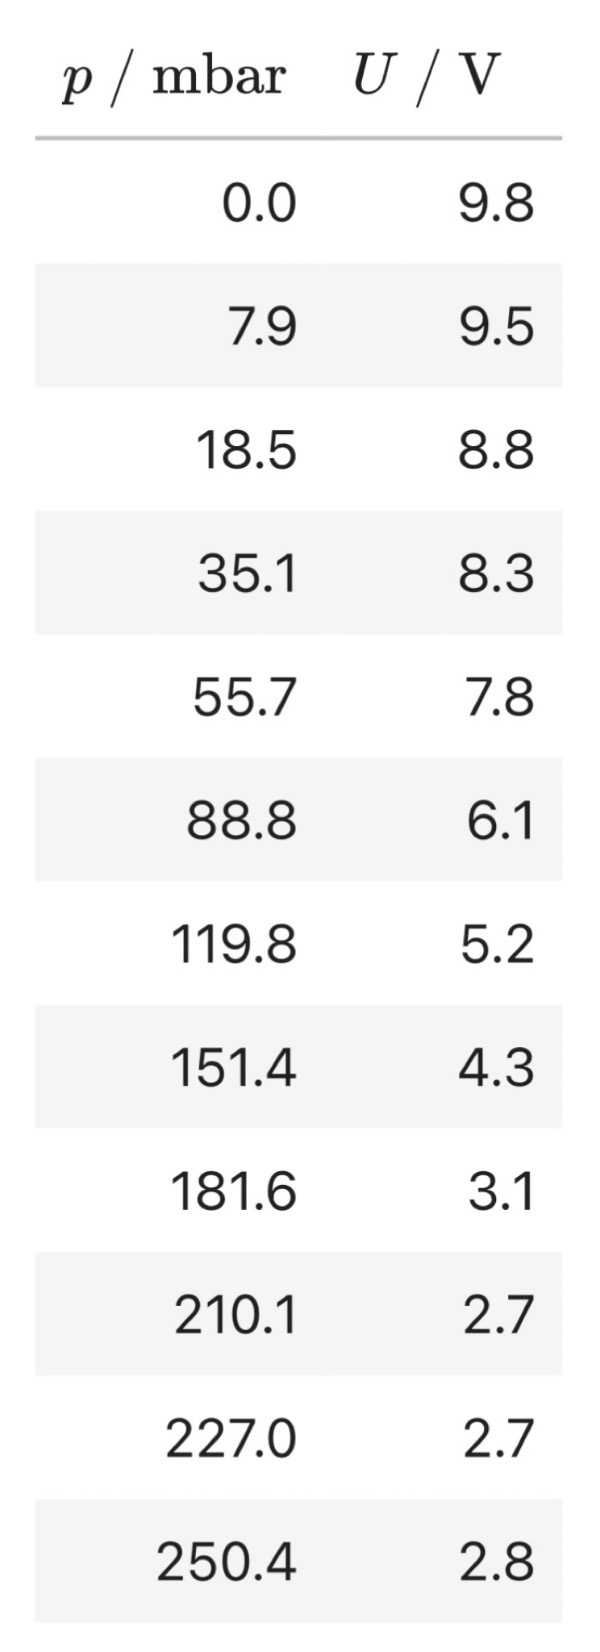
\includegraphics[width=\textwidth]{content/tabelle/OhneFolie.jpg}
    	\label{tab:OhneFolie}
	\end{subfigure}
	\hfill
	\begin{subfigure}{0.18\textwidth}
    	\centering
    	\caption{Mit Folie.}
    	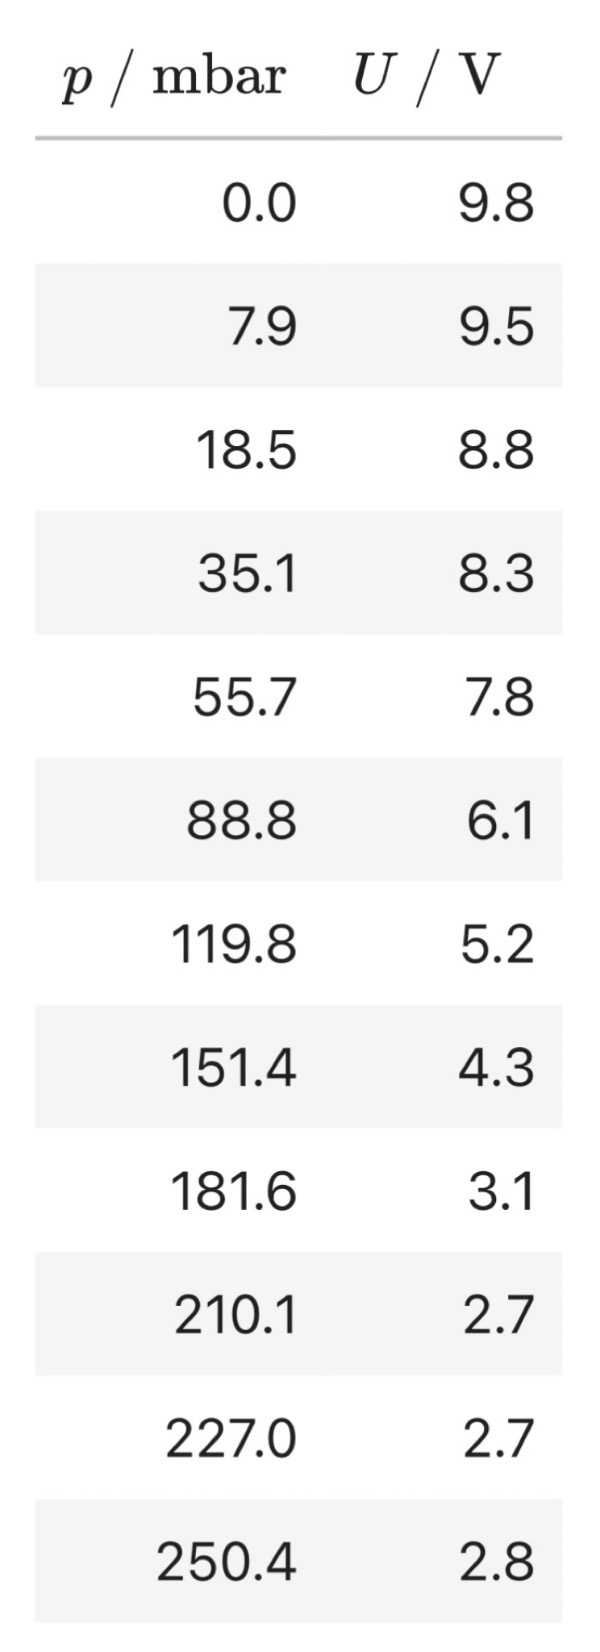
\includegraphics[width=\textwidth]{content/tabelle/MitFolie.jpg}
    	\label{tab:MitFolie}
	\end{subfigure}
	\hspace{9em}
\end{table}

\begin{figure}[H]
    \centering
    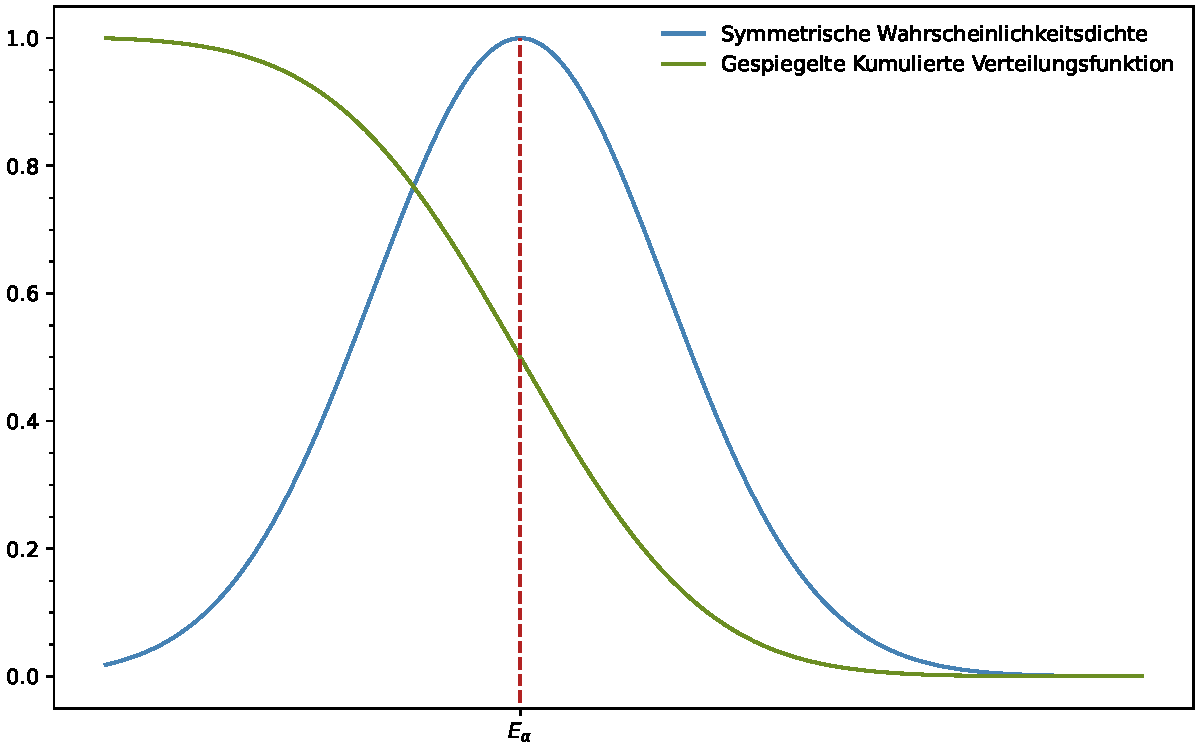
\includegraphics[width=0.963\textwidth]{content/messung/Energieverteilung.pdf}
    \caption{Normierte repräsentative Energieverteilungen der Alphastrahlung.}
    \label{fig:Energieverteilung}
\end{figure}

\begin{figure}[H]
    \centering
    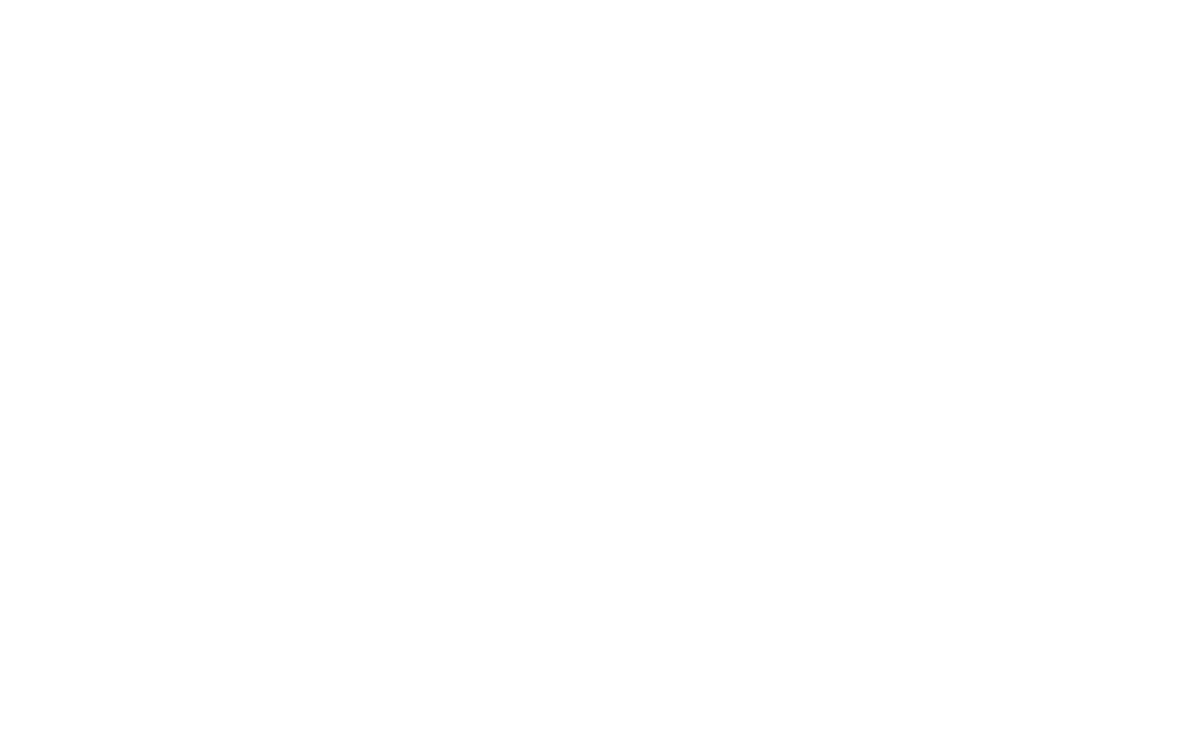
\includegraphics[width=\textwidth]{content/messung/Golddicke.pdf}
    \caption{Lineare Regressionen der Maximalspannungen $U$ in Abhängigkeit des Drucks $p$ mit und ohne Goldfolie.}
    \label{fig:Golddicke}
\end{figure}

Die in Abbildung \ref{fig:Golddicke} aufgetragenen Messwerte werden um die farblich hervorgehobenen Daten bei höheren Drücken wegen zu hohem
Rauschen bereinigt, um anschließend eine lineare Ausgleichsrechnung auszuführen. Die Funktion sowie die Umkehrung lauten also
\begin{align*}
	&&&& U = ap + b && \text{und} && p = \pfrac{U - b}{\raisebox{0.5ex}{$a$}} &&&&
\end{align*}
\vspace{-2em}
\begin{align*}
	& \text{mit} & a_\text{of} &= \qty{-0.0368+-0.0008}{\volt\per\milli\bar} &&
	\text{und} & b_\text{of} &= \qty{12.10+-0.12}{\volt} && \text{ohne Folie} \\
	& \text{sowie} & a_\text{mf} &= \qty{-0.0364+-0.0010}{\volt\per\milli\bar} &&
	\text{und} & b_\text{mf} &= \qty{9.65+-0.10}{\volt} && \text{mit Folie} \vspace{-2em}
\end{align*}
als Parameter aus der Regressionsrechnung. Damit und mit $U_\alpha = \qty{6.05}{\volt}$ ergeben sich $p_\alpha = \qty{165+-5}{\milli\bar}$
und $\Delta p = \qty{66+-6}{\milli\bar}$ sowie schließlich
\begin{equation*}
	\Delta E = \qty{2.2+-0.2}{\mega\electronvolt}
\end{equation*}
für die Energiedifferenz. Gleichung \eqref{eqn:Bethe} lässt sich dann zu
\begin{equation*}
	d = \Delta x = \Delta E \frac{4\pi m_e v_\alpha^2 \varepsilon_0^2}{e^4 N z^2 Z \ln (2m_e v_\alpha^2 / I)}
	= \Delta E \frac{8\pi m_e E_\alpha \varepsilon_0^2}{m_\alpha e^4 N z^2 Z \ln (4m_e E_\alpha / m_\alpha I)} =
	\qty{5.1+-0.4}{\micro\meter}
\end{equation*}
umstellen. Hier wird $I_G = Z_G \qty{10}{\electronvolt} = \qty{790}{\electronvolt}$ als Anregungspotential genähert.
\subsection*{Streuwinkelabhängigkeit}

Zählrate $C$ und Fehler $\Delta C$ lassen sich aus den Messdaten in Tabelle \ref{tab:Streuwinkel} mit
\begin{align*}
	&&&& C = \pfrac{\mathscr{C}}{t} && \text{und} && \Delta C = \pfrac{\sqrt{\mathscr{C \,}}}{t} &&&&
\end{align*}
berechnen, wobei eine Poissonverteilung angenommen wird. Die Beziehung
\begin{equation*}
	\sigma = \pfrac{C}{A} \, \pfrac{F}{\mathscr{N}}
\end{equation*}
für den Wirkungsquerschnitt, der die Zahl $\mathscr{N} \kern-0.3pt = NV$ von Streuzentren im Volumen $V \kern-0.3pt = dF$ enthält,
deutet im Vergleich mit \eqref{eqn:Rutherford} auf einen $C \propto \sin^{-4}(\vartheta / 2)$ Zusammenhang hin.

\begin{table}[H]
    \centering
    \caption{Messdaten der Zählrate in Abhängigkeit vom Streuwinkel.}
    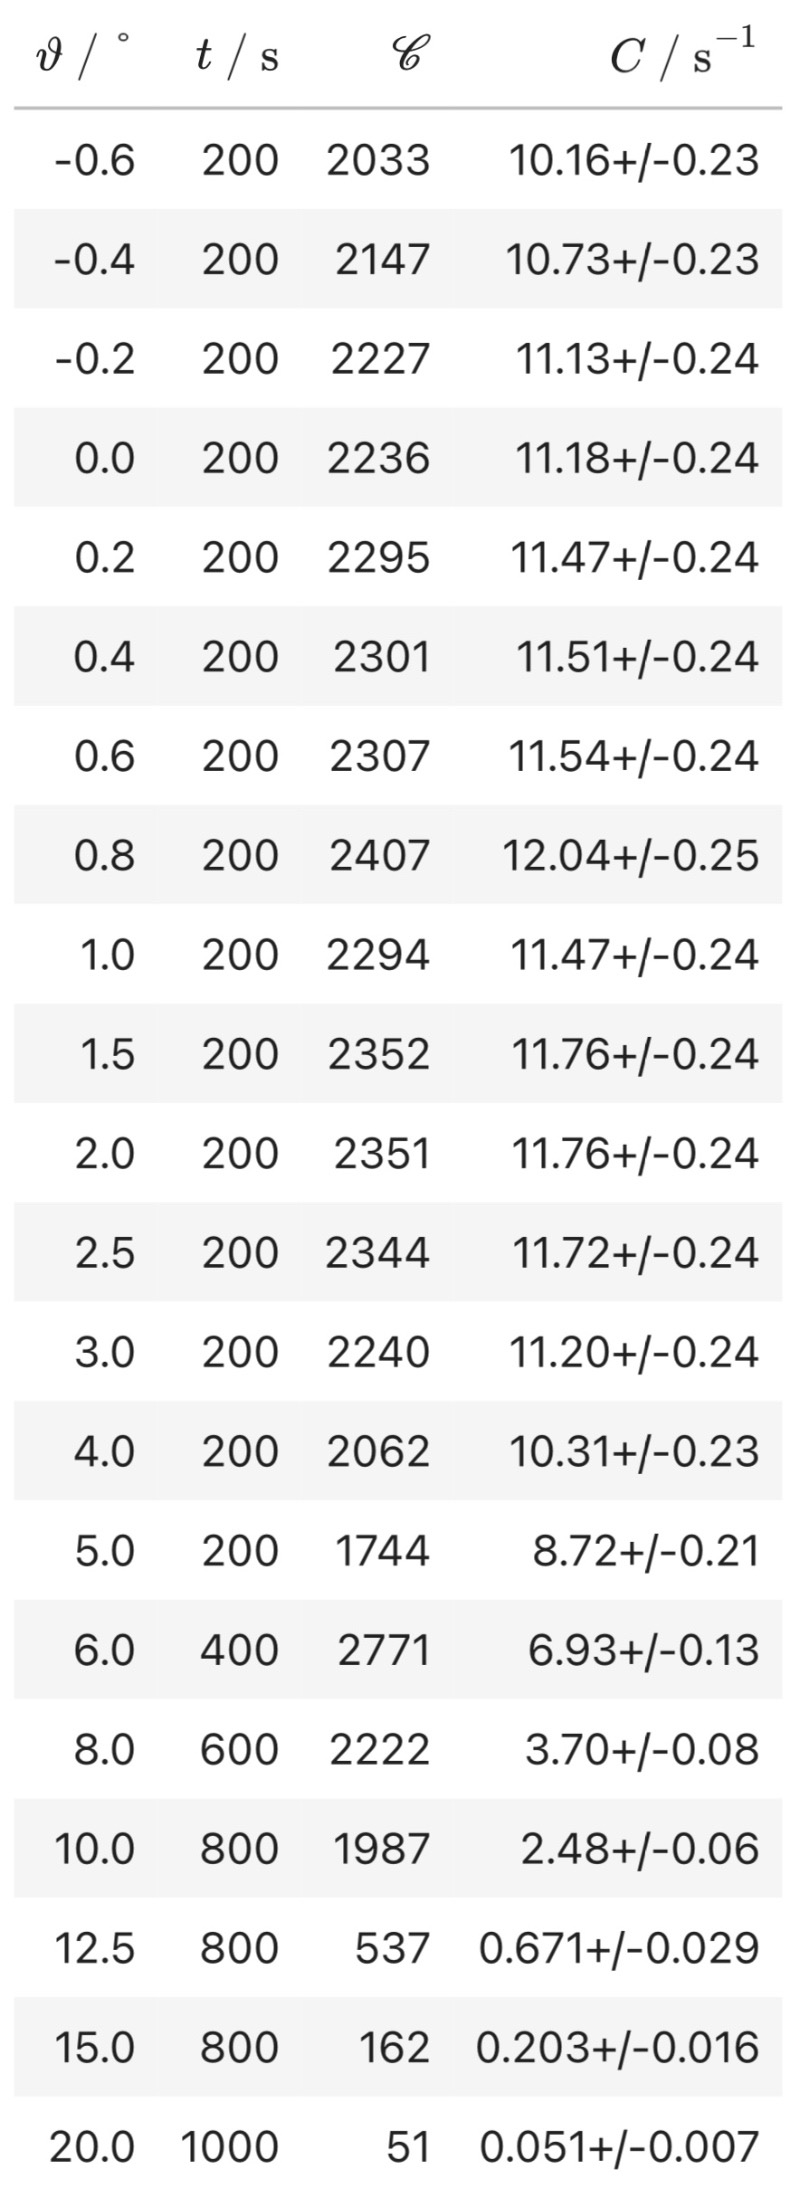
\includegraphics[width=0.32\textwidth]{content/tabelle/Streuwinkel.jpg}
    \label{tab:Streuwinkel}
\end{table}

\begin{figure}[H]
    \centering
    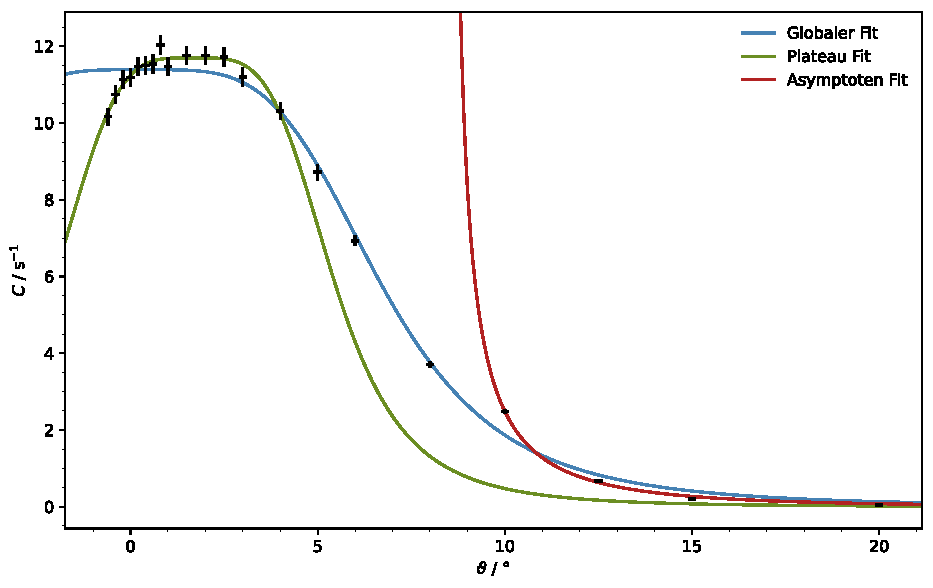
\includegraphics[width=\textwidth]{content/messung/Streuwinkel.pdf}
    \caption{Winkelabhängigkeit der Zählrate mit verschieden parametrisierten Fits.}
    \label{fig:Streuwinkel}
\end{figure}

Um diese Abhängigkeit zu untersuchen, wird eine modifizierte Funktion der Form
\begin{equation*}
	C = \pfrac{a}{\sin^4 \bigl( (\vartheta - b) / 2 \bigr) + c}
\end{equation*}
mir drei Freiheitsgraden angesetzt. Dabei gibt $a$ Asymptote und Skalierung an, der Parameter $b$ erlaubt eine Verschiebung des Maximumwinkels
und $c$ dient zur Korrektur der Singularität auf einen Peak endlicher Höhe. Als Test werden mehrere nichtlineare Ausgleichsrechnungen
vorgenommen, global an alle Messwerte, an die ersten 14 Werte des Plateaus, und an die letzten 4 Werte der Asymptote. Es ergeben sich
\begin{align*}
	a_\text{glob} &= \qty{1.1+-0.4e-4}{\per\second} & b_\text{glob} &= \qty{3+-5}{\degree} & c_\text{glob} &= \num{10+-3e-6} \\
	a_\text{plat} &= \qty{1.4+-0.1e-5}{\per\second} & b_\text{plat} &= \qty{1.69+-0.05}{\degree} & c_\text{plat} &= \num{1.2+-0.1e-6} \\
	a_\text{asym} &= \qty{7e-5}{\per\second} & b_\text{asym} &= \qty{2e-9}{\degree} & c_\text{asym} &= \num{-3e-5} \vspace{-2em}
\end{align*}
als Koeffizienten, wobei der asymptotische Fit keine stabile Konvergenz zeigt und dadurch keine Kovarianz geschätzt werden kann.
